%%%%%%%%%%%%%%%%%%%%%%%%%%%%%%%%%%%%%%%%%%%%%%%%%%%%%%%%%%%%
% standard header
    \documentclass[aspectratio=169]{beamer}
    \mode<presentation>
%%%%%%%%%%%%%%%%%%%%%%%%%%%%%%%%%%%%%%%%%%%%%%%%%%%%%%%%%%%%
% color stuff
    \usetheme{AnnArbor}
    \usecolortheme[accent=blue]{solarized}
    \colorlet{solarizedMixFg}{solarizedRebase2!80!solarizedRebase0}
    \setbeamercolor{normal text}{fg=solarizedMixFg, bg=solarizedRebase02}
    \setbeamercolor{palette primary}{fg=solarizedMixFg, bg=solarizedRebase01}
    \setbeamercolor{palette secondary}{fg=solarizedMixFg, bg=solarizedRebase01}
    \setbeamercolor{palette tertiary}{fg=solarizedMixFg, bg=solarizedRebase01}
    \setbeamercolor{palette quaternary}{fg=solarizedMixFg, bg=solarizedRebase01}
%%%%%%%%%%%%%%%%%%%%%%%%%%%%%%%%%%%%%%%%%%%%%%%%%%%%%%%%%%%%
% font stuff
    \usepackage{hejohns-fonts}
    \usefonttheme{serif}
%%%%%%%%%%%%%%%%%%%%%%%%%%%%%%%%%%%%%%%%%%%%%%%%%%%%%%%%%%%%
% packages
    \usepackage{tikz}
    \usepackage{tikz-cd}
    \usetikzlibrary{positioning}
    \usepackage{graphicx}
    \usepackage{media9}
    \usepackage{svg}
%%%%%%%%%%%%%%%%%%%%%%%%%%%%%%%%%%%%%%%%%%%%%%%%%%%%%%%%%%%%
\begin{document}
%\beamertemplatenavigationsymbolsempty
\setbeamertemplate{navigation symbols}{}
%\setbeamercolor{button}{bg=blue, fg=white}
\title[Judgmental Reconstruction]{Modal Logic}
\subtitle{subtitle: TBD}
\author{hejohns}
\date{\today}
\titlegraphic{\fbox{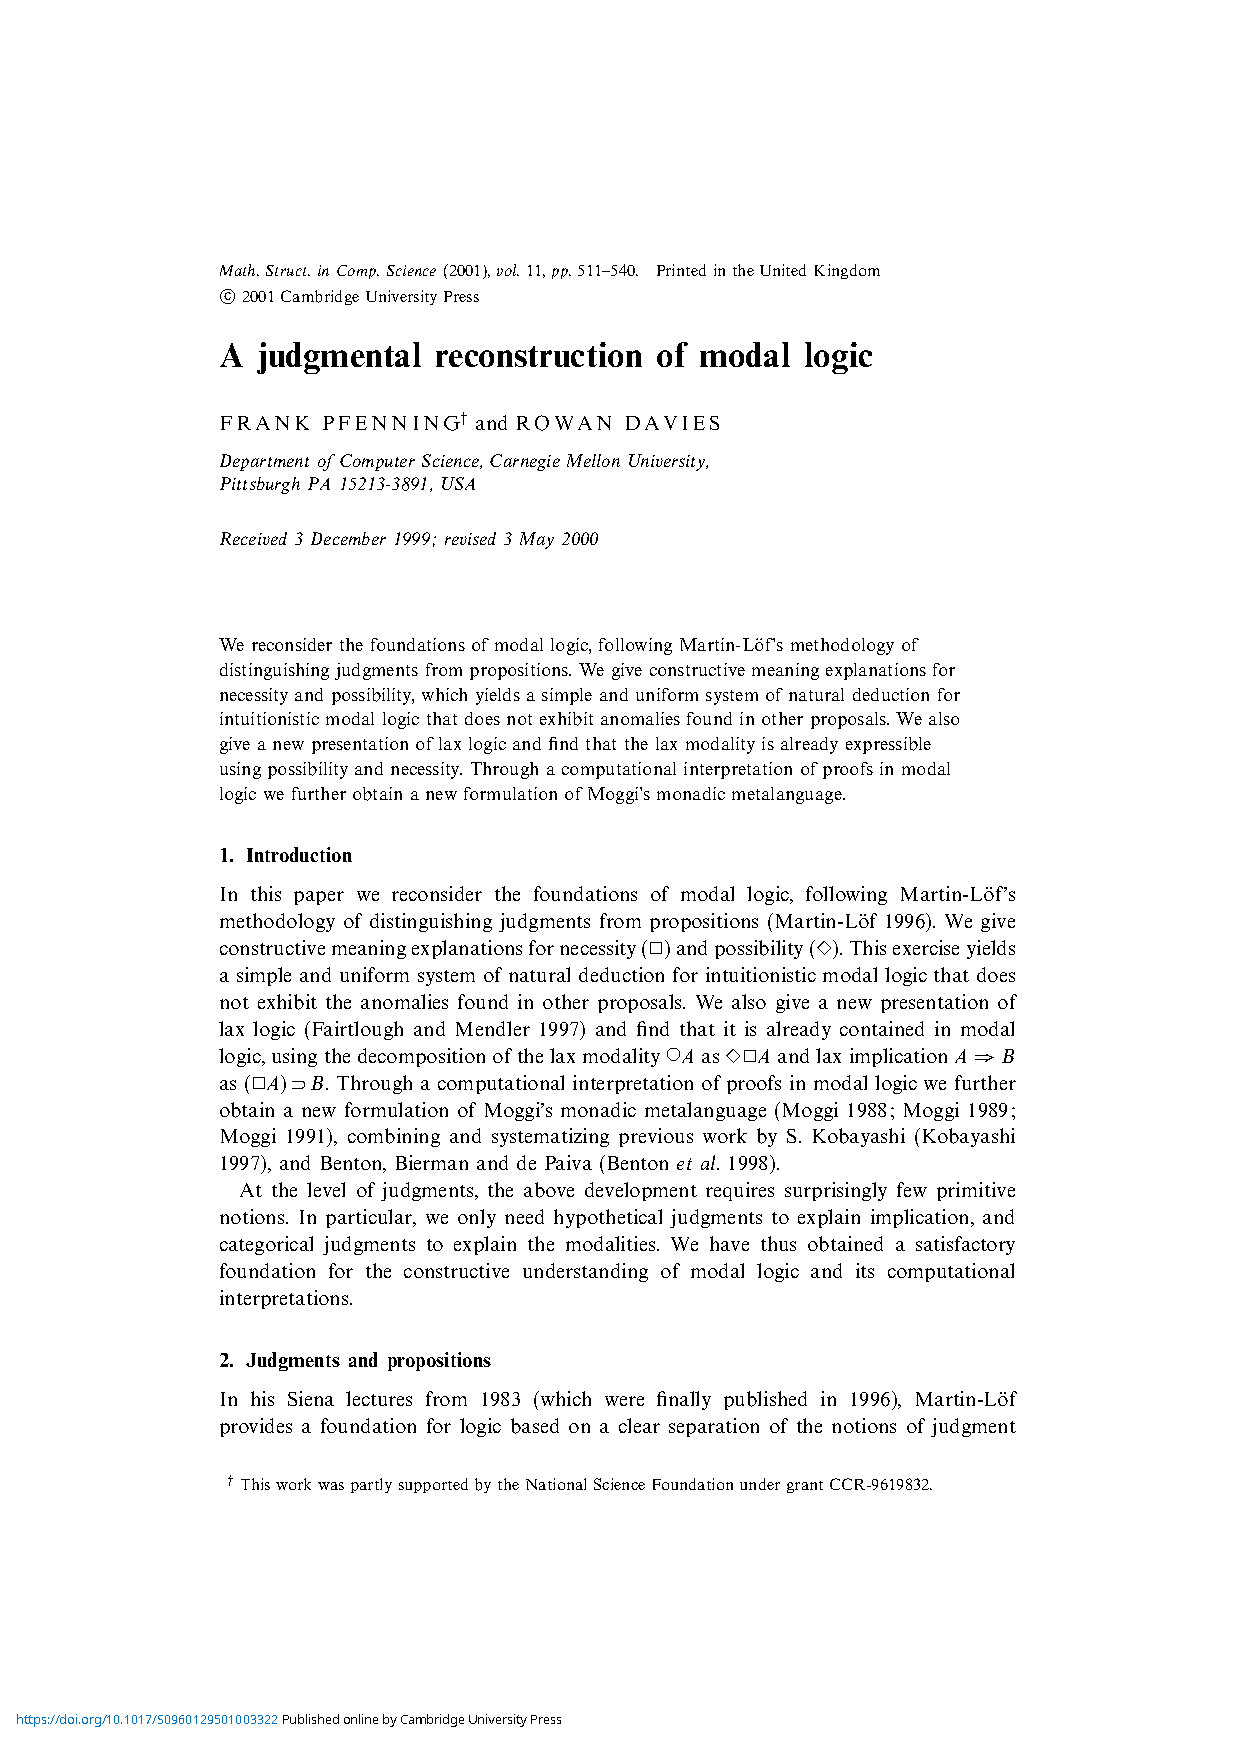
\includegraphics[page=1,scale=0.6,clip,trim=2.5cm 9cm 5.2cm 4.4cm]{jr.pdf}}}
\begin{frame}
    \titlepage
\end{frame}
\section{Kripke Semantics}
\begin{frame}
    \frametitle{About}
    $λ$Π
\end{frame}
\begin{frame}
    \begin{tikzpicture}[commutative diagrams/.cd, every diagram, scale=4]
        \begin{scope}[node distance=1 and 1]
            \node[](K) at (0, 0){$K$};
            \node[above=of K](D){$D$};
            \node[above=of D](M){$M$};
            \node[above right=0.6 and 0.2 of K](K4){$K4$};
            \node[above right=0.2 and 0.9 of K](K5){$K5$};
            \node[above right=0.1 and 0.45 of K5](K45){$K45$};
            \node[above=of K4](D4){$D4$};
            \node[above=of D4](S4){$S4=M4$};
            \node[right=2 of K](KB){$KB$};
            \node[above right=0.6 and 0.2 of KB](KB5){$KB5$};
        \end{scope}
        \draw[commutative diagrams/.cd, every label]
        (D)edge(M)
        (K)edge(D)
        (K)edge(K4)
        (K)edge(KB)
        ;
    \end{tikzpicture}
\end{frame}
\section{References}
\begin{frame}[allowframebreaks]
    \frametitle{References}
    \begin{thebibliography}{00}
        \setbeamertemplate{bibliography item}{\insertbiblabel}
        \bibitem{sourceA}
        TODO: ask me
    \end{thebibliography}
\end{frame}
\end{document}
